\subsubsection{UC9 - Coniazione Cubit}
\begin{itemize}
	\item \textbf{Attori Primari}: governo;
	\item \textbf{Attori Secondari}: MetaMask\glo;
	\item \textbf{Descrizione}: viene coniata una quantità definita di Cubit\glo;
	
	\item \textbf{Scenario principale}: il governo ritiene necessario coniare ulteriori Cubit\glosp rispetto a quelli attualmente presenti sul mercato. Per fare ciò deve accedere alla pagina dedicata in cui, attraverso un form dovrà:
	 \begin{enumerate}[label=\alph*.]
		\item inserire la quantità di Cubit \texttt{x} da coniare;
		\item confermare tale operazione attraverso l'utilizzo di MetaMask\glo;
	\end{enumerate}
	\item \textbf{Precondizione}: siano \texttt{x} i Cubit\glosp che il governo vuole coniare e \texttt{n} i Cubit\glosp attualmente in circolo. L'utente governativo è acceduto alla pagina per la coniazione ed ha compilato e confermato il form;
	\item \textbf{Postcondizione}: i Cubit\glosp in circolo sono \texttt{n+x}.
\end{itemize}
\subsubsection{UC10 - Distribuzione Cubit}
%non capisco perchè la figura è prima del titolo sul PDF
\begin{figure}[h]
	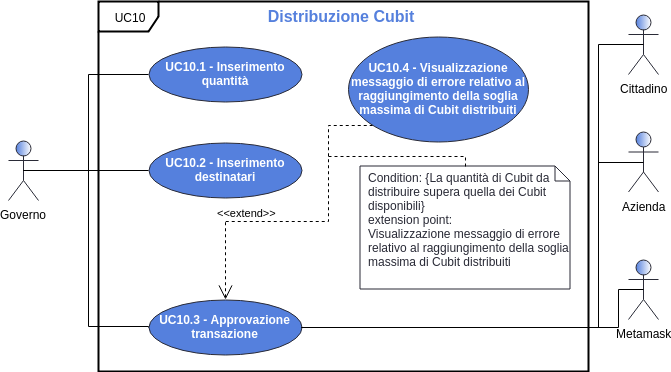
\includegraphics[width=13.5cm]{res/images/UC10Distribuzione.png} %da adattare in larghezza
	\centering
	\caption{UC10 - Distribuzione Cubit}
	
\end{figure}
\begin{itemize}
	\item \textbf{Attori Primari}: governo;
	\item \textbf{Attori Secondari}: MetaMask\glo, cittadino, azienda\glo;
	\item \textbf{Descrizione}: il governo versa una quantità di Cubit\glosp sull'account di uno o più  utenti, che siano essi cittadini o aziende. Questi ricevono la quantità di Cubit\glosp definita da parte del governo;
	\item \textbf{Scenario}: il governo clicca sull'apposito pulsante per distribuire una somma di Cubit definita, ad uno o più utenti specificati; 
	\item \textbf{Precondizione}: il governo viene notificato di dover distribuire una quantità specifica di Cubit\glosp ad uno o più utenti specifici;
	\item \textbf{Postcondizione}: tali utenti ricevono i Cubit\glosp da parte del governo.
\end{itemize}
\subsubsection{UC10.1 - Inserimento quantità}
\begin{itemize}
	\item \textbf{Attori Primari}: governo;
	\item \textbf{Descrizione}: il governo inserisce nell'apposito form la quantità di Cubit\glosp da distribuire, ritenendo la quantità inserita come quantità da inviare ad ogni singolo utente;
	\item \textbf{Scenario}: il governo inserisce una quantità \texttt{x} di Cubit\glosp da inviare;
	\item \textbf{Precondizione}: il governo sa quanti Cubit\glosp deve distribuire ad ogni singolo utente;
	\item \textbf{Postcondizione}: il governo può procedere a selezionare gli utenti desiderati.
\end{itemize}
\subsubsection{UC10.2 - Inserimento destinatari}
\begin{itemize}
	\item \textbf{Attori Primari}: governo;
	\item \textbf{Attori Secondari}: cittadino, azienda;
	\item \textbf{Descrizione}: il governo inserisce nell'apposito form la lista di destinatari che intendono ricevere la quantità di Cubit\glosp precedentemente inserita;
	\item \textbf{Scenario}: il governo inserisce una lista di destinatari;
	\item \textbf{Precondizione}: il governo sa quanti e quali utenti riceveranno la somma di Cubit\glosp selezionata, è necessario quindi aver inserito una quantità di Cubit\glosp da distribuire;
	\item \textbf{Postcondizione}: il governo può procedere ad approvare la transazione.
\end{itemize}
\subsubsection{UC10.3 - Approvazione transazione}
\begin{itemize}
	\item \textbf{Attori Primari}: governo;
	\item \textbf{Attori Secondari}: MetaMask\glo, cittadino, azienda\glo;
	\item \textbf{Descrizione}: il governo decide se approvare o rifiutare la transazione;
	\item \textbf{Scenario}: il governo ha appena inserito una quantità \texttt{x} di Cubit\glosp da distribuire ad ogni singolo utente e ha pure selezionato una lista di \texttt{y} utenti;
	\item \textbf{Estensioni}:
	\begin{itemize}
		\item \textbf{UC10.4}: il governo vedrà un messaggio di errore se \texttt{x*y} supera la quantità di Cubit\glosp disponibili alla distribuzione;
	\end{itemize}
	\item \textbf{Precondizione}: è necessario aver selezionato una lista di utenti e una quantità da distribuire ad ogni singolo utente;
	\item \textbf{Postcondizione}: ogni utente riceverà nel proprio wallet\glosp la quantità di Cubit\glosp distribuita dal governo.
\end{itemize}
\subsubsection{UC10.4 - Visualizzazione messaggio di errore relativo al raggiungimento della soglia massima di Cubit\glosp distribuiti}
\begin{itemize}
	\item \textbf{Attori Primari}: governo;
	\item \textbf{Descrizione}: il governo riceve un messaggio di errore relativo al fatto che ha selezionato una quantità di Cubit\glosp superiore a quella disponibile alla distribuzione;
	\item \textbf{Scenario}: il governo clicca sull'apposito pulsante per confermare la transazione di distribuzione ma non ha sufficienti fondi per completare tale operazione;
	\item \textbf{Precondizione}: il governo deve aver inserito una quantità di Cubit\glosp superiore a quella disponibile;
	\item \textbf{Postcondizione}: il governo ora è a conoscenza del fatto che se vorrà distribuire la somma selezionata, dovrà avere sufficienti fondi.
	
\end{itemize} 
